\section{Evaluation}

\begin{frame}
  \frametitle{Evaluation}
\begin{itemize}

	\item We wanted to rigorously compare our results with the results from the original paper.
	\item But: no implicit datasets available!

	\item We had to implement a special random number generator (RNG) and a benchmark generator from pseudocode delivered by \cite{Benchmarks}.

	\item The benchmarks were reproduced based on given seeds for the RNG.
\end{itemize}

\end{frame}

%%%%%%%%%%%%%%%%%%%%%%%%%%%%%%%%%%%%%%%%%%%%%%%%%%%%%%%%%%%%%%%%%%%%%%%%%%%%%%%%

\begin{frame}
	\frametitle{Evaluation method}
\begin{itemize}

	\item We considered benchmark problems of sizes 4x4 (4 jobs, 4 machines), 5x5, 7x7, 10x10, 15x15, 20x20. 
	For each problem, we  ran all 3 algorithms for 200 generations (500 in original paper) with a population size of 200.

	\item 	Since different runs produce different results, we repeated each run 100 times. 
	\\ 		\textrightarrow		High computational cost!

	\item 	Complexity increases with rising problem size \textrightarrow	only a few large problems evaluated 
\end{itemize}

	
\end{frame}

%%%%%%%%%%%%%%%%%%%%%%%%%%%%%%%%%%%%%%%%%%%%%%%%%%%%%%%%%%%%%%%%%%%%%%%%%%%%%%%%

\begin{frame}
  \frametitle{Results}
\begin{figure}[htbp]
	\centering
		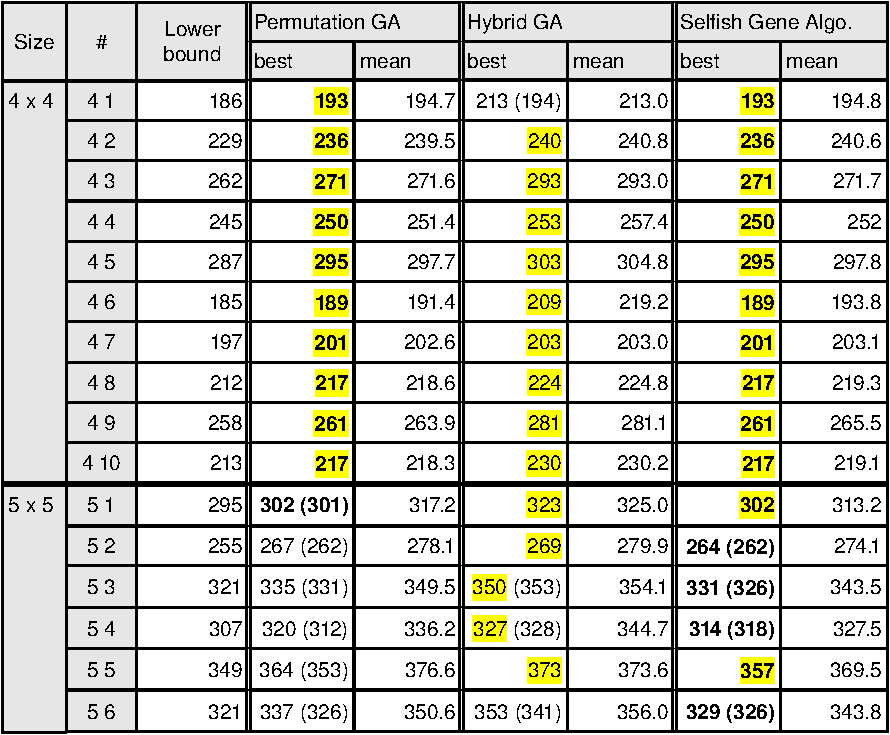
\includegraphics[scale=.5]{images/results1.pdf}
	\caption{caption}
	\label{fig:label}
\end{figure}
\end{frame}

%%%%%%%%%%%%%%%%%%%%%%%%%%%%%%%%%%%%%%%%%%%%%%%%%%%%%%%%%%%%%%%%%%%%%%%%%%%%%%%%

\begin{frame}
  \frametitle{Results (2)}
\begin{figure}[htbp]
	\centering
		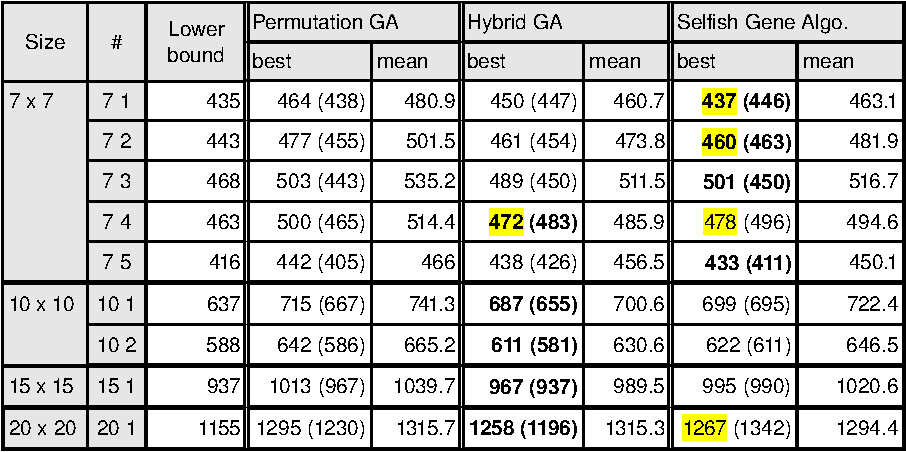
\includegraphics[scale=.5]{images/results2.pdf}
	\caption{caption}
	\label{fig:label}
\end{figure}
\end{frame}


\begin{frame}
  \frametitle{Convergence}
\end{frame}

\begin{frame}
  \frametitle{Comparison}
\end{frame}